\documentclass[11p]{article}
\usepackage[a4paper, total={5.5in, 9in}]{geometry}
\usepackage[leqno]{amsmath}
\usepackage{tikz}
\makeatletter
\newcommand{\leqnomode}{\tagsleft@true\let\veqno\@@leqno}
\newcommand{\reqnomode}{\tagsleft@false\let\veqno\@@eqno}
\makeatother
\usepackage{amssymb}
\usepackage{amsthm}
\usepackage{float}
\usepackage{bbm}
\usepackage{color}
\usepackage{multirow}
\usepackage{booktabs}
\usepackage{algpseudocode}
\usepackage{rotating}
\usepackage{titling}
\usepackage{authblk} %new
\usepackage{blindtext} %new
\usepackage{breakcites} %break logn citationa
\providecommand{\keywords}[1]{\textbf{\textit{Keywords---}} #1} %keywords
\usepackage[toc,page]{appendix} %appendix package
\usepackage{algorithm}
\usepackage{hyperref}

\newtheorem{theorem}{Theorem}
\newtheorem{proposition}{Proposition}
\theoremstyle{definition}
\theoremstyle{definition}
\newtheorem{remark}{Remark}
\theoremstyle{theorm}
\newtheorem{lemma}{Lemma}
\newtheorem{corollary}{Corollary}

\newtheorem{definition}{Definition}
\allowdisplaybreaks

\begin{document}
\setlength{\droptitle}{-4em}   % This is your set screw

\title{Identifying responsibility in a Nigerian sex trafficking network: A game theoretical approach}
%\author{Frank de Meijer \qquad Aras Selvi }
%\author{Aras Selvi}
%\affil{CentER, Department of Econometrics and OR, Tilburg University, The Netherlands }
\author[1]{Frank de Meijer}
\author[2]{Aras Selvi}
\affil[ ]{ CentER, Department of Econometrics and OR, Tilburg University, The Netherlands}
\affil[1]{\textit {\href{mailto:f.j.j.demeijer@tilburguniversity.edu}{f.j.j.demeijer@tilburguniversity.edu}}}
\affil[2]{\textit {\href{mailto:a.selvi@tilburguniversity.edu}{a.selvi@tilburguniversity.edu}}}

%\date{\today}
\date{}

\maketitle

\begin{abstract} \noindent
In this work, we investigate a popular network problem arising in the criminal sciences as well as psychological studies. We are given a Nigerian sex trafficking network, and we are interested in finding the most effective members in this network. However, the definition of effectiveness is vague in most cases, since a member who connects a lot of criminals can be as dangerous as someone who `owns' many victims. Therefore, we introduce a game theoretical setting to this problem, and by using Operations Research techniques we approximate the Shapley value: a measure of importance of a `player' in a cooperative game, considering every possible coalitions. 
\end{abstract}
\keywords{Shapley value, connectivity games, human trafficking networks}

\reqnomode

\section{Introduction}
Thousands of West-African sex-trafficking victims are arriving to Europe every year \cite{morselli2009inside}. Moreover, \cite{olagbegi2006human} shows that most of these victims are from Nigeria, since the majority of crime networks in Nigeria are based on sex-trafficking for various reasons (unemployment, persuasion via rituals, threatening, etc.). The paper \cite{mancuso2014not} studies a network in Nigerian sex-trafficking, which obtains its data $\ldots$
\section{Game Theoretical Setting}
Let $M$ denote the set of madams and let $C$ denote the set of controllers. For all $i \in N$, let $d_i$ denote the number of victims for which player $i$ is directly responsible. A network can be interpreted as an undirected graph $G = (N,E)$ with vertex set $N$ and edge set $E$. To each player we assign exactly one vertex in $N$. For our case, this implies that $N = M \cup C$. If two players communicate, we connect their corresponding vertices by an edge. For each subset $S \subseteq N$, let $G[S] = (N[S], E[S])$ denote the subgraph of $G$ induced by the players in $S$. To each player $i \in N$ we assign a non-negative weight $w_i \in \mathbb{R}$. This weight represents the direct responsibility of the player in the network. 

A cooperative game is represented by the pair $(N,v)$, where $N$ equals the set of players and the function $v : 2^N \rightarrow \mathbb{R}$ assigns a value to each coalition $S \subseteq N$. The value $v(S)$ can be seen as a measure for the effectiveness of the subnetwork induced by the players in $S$. The value of the grand coalition, $v(N)$, can be seen as the total effectiveness of the network. The Shapley value \cite{shapley1953value} is a solution concept that allocates $v(N)$ among the set of players based on the players' marginal contributions to the coalitions. If some player is assigned a high value, it has a high influence on the effectiveness of the network. Hence, the Shapley value can be used as a game theoretical centrality measure of the network.

The main question is how to define $w$ and $v$ such that they represent the effectiveness of a coalition in the best way. We propose two settings. 

In general, the madams are directly responsible for the victims, while the controllers only operate as intermediates. To model this direct responsibility, we define the weight function $w^\alpha$ in the following way:
\begin{align*}
    w^\alpha_i = \begin{cases} d_i & \text{if $i \in M$,} \\d_i + 
    \alpha \sum_{j \in M : (i,j) \in E}d_j & \text{otherwise,}
    \end{cases}
\end{align*}
where $\alpha \in [0,1]$ is a parameter which we call the control parameter. This parameter indicates the indirect responsibility of the controllers in the network. If $\alpha = 0$, the controllers are considered responsible for the victims only indirectly, whereas $\alpha = 1$ indicates that the controllers are directly responsible for all victims of neighbouring players. Now, for every coalition $S$ we define
\begin{align*}
    v(S) = \max_{\substack{T \subseteq S : T \\ \text{connected}}}\quad \sum_{i \in T}w^\alpha_i. 
\end{align*}
One can easily verify that the corresponding game $(N, v)$ is monotonic for all $\alpha \in [0,1]$. Namely, if $S_1 \subset S_2$ and $T$ is the largest weighted connected component in $S_1$, then also $T \subseteq S_2$. Consequently, we know that $v(S_2) \geq \sum_{i \in T}w^\alpha_i = v(S_1)$.
\section{Computation and Results}

\section{Sensitivity Analysis}


\section{Discussion}

\bibliographystyle{apalike}
\bibliography{sample}
\newpage
\begin{appendices}
\section{Network Figure}   
\begin{figure}[ht]
\centering
    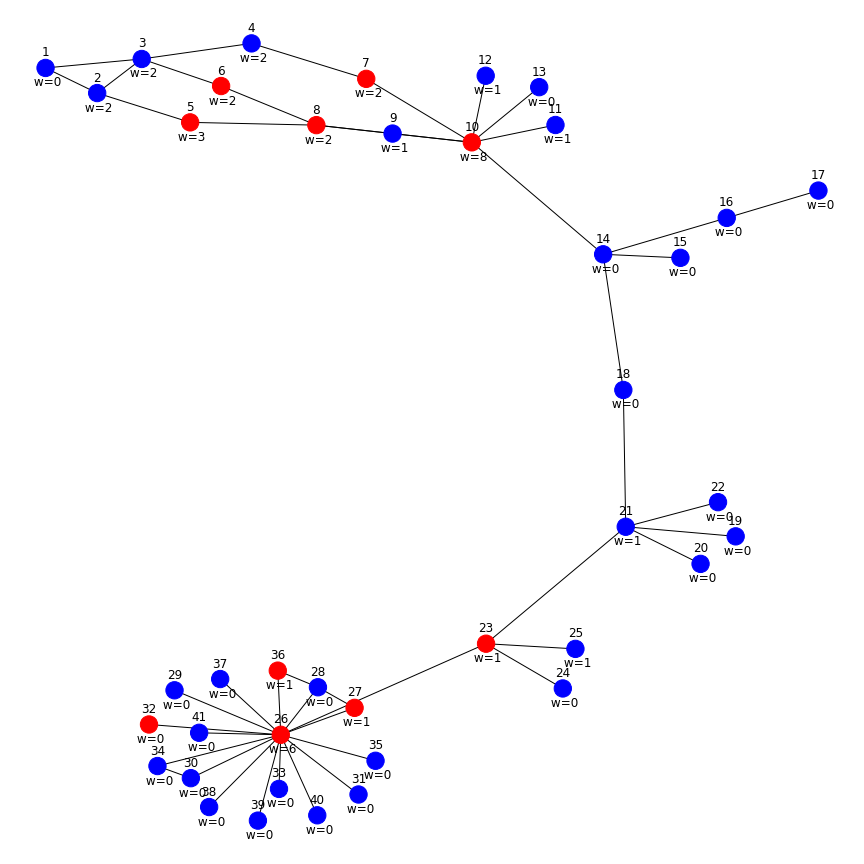
\includegraphics[angle=0,scale=0.5]{network.png}%<---angle here
    \caption{Sex trafficking network. Blue nodes are `responsible for control', red nodes are `madams'. Node indexes are written above a node, while the weight is written just below the node in form $w=$.}
    \label{fig:PropProf}
\end{figure}
\end{appendices}

\end{document}